\documentclass[11pt]{article}

\usepackage{enumitem}


%%TO EDIT
\newcommand{\dueclassnumber}{37}
\newcommand{\assignmentnum}{15}

% CHANGE issolution{0} to issolution{1} for homework submission.
% WRITE solutions inside the \solution{} commands.
% or, you can use \if\issolution1 … \fi

\def\issolution{1}
\def\myname{Allen Liu} % My name goes here
\def\mysec{01} % Section number goes here
\def\myCM{374} % Campus Mailbox goes here

\input{../common/flags}

% Leave the next line alone. This is for my answer keys.
%\def\isanswerkey{1}

\usepackage{bbm,fancyhdr,ifthen,setspace,hyperref,url}
\usepackage{amssymb,amsmath,enumitem,amsthm,mathrsfs}
\usepackage{graphicx,xspace,color}
\usepackage{hhline}
\usepackage{tikz}
\usetikzlibrary{automata, positioning, arrows,chains,scopes,fit}
\tikzset{
->, % makes the edges directed
>=stealth', % makes the arrow heads bold
node distance=2.4cm, % specifies the minimum distance between two nodes. Change if necessary.
every state/.style={thick, fill=gray!10}, % sets the properties for each ’state’ node
initial text=$ $, % sets the text that appears on the start arrow
}

\topmargin=-.5in
\headsep=0.0in
\oddsidemargin=-.35in
\evensidemargin=-.65in
\textwidth=7.25in
\textheight=9.75in
\footskip=0in
\usepackage{titlesec}
\titlespacing*{\paragraph}{0pt}{2ex plus 1ex minus .2ex}{1ex}
\fancyhf{} % clear all header and footers
\renewcommand{\headrulewidth}{0pt} % remove the header rule
%\rfoot{\thepage}
\pagestyle{fancy}

\ifx\myname\undefined
\def\myname{}
\fi

\ifx\isanswerkey\undefined
\def\isanswerkey{0}
\fi

\if\isanswerkey1
\def\issolution{1}
\fi


\newcommand{\getcourseyear}[1]{2022}
\newcommand{\getcourseterm}{Spring \getcourseyear{1}}

\newcommand{\getclassmonthnum}[1]{\ifthenelse{#1<16}{3}{\ifthenelse{#1<29}{4}{5}}}
\newcommand{\getclassmonthshort}[1]{\ifthenelse{#1<16}{Mar}{\ifthenelse{#1<29}{Apr}{May}}}
\newcommand{\getclassmonth}[1]{\ifthenelse{#1<16}{March}{\ifthenelse{#1<29}{April}{May}}}
\newcommand{\getclassdayofmonth}[1]{\ifthenelse{
#1=1}{7}{\ifthenelse{
#1=2}{8}{\ifthenelse{
#1=3}{10}{\ifthenelse{
#1=4}{11}{\ifthenelse{
#1=5}{14}{\ifthenelse{
#1=6}{15}{\ifthenelse{
#1=7}{17}{\ifthenelse{
#1=8}{18}{\ifthenelse{
#1=9}{21}{\ifthenelse{
#1=10}{22}{\ifthenelse{
#1=11}{24}{\ifthenelse{
#1=12}{25}{\ifthenelse{
#1=13}{28}{\ifthenelse{
#1=14}{29}{\ifthenelse{
#1=15}{31}{\ifthenelse{
#1=16}{1}{\ifthenelse{
#1=17}{4}{\ifthenelse{
#1=18}{5}{\ifthenelse{
#1=19}{7}{\ifthenelse{
#1=20}{8}{\ifthenelse{
#1=21}{18}{\ifthenelse{
#1=22}{19}{\ifthenelse{
#1=23}{21}{\ifthenelse{
#1=24}{22}{\ifthenelse{
#1=25}{25}{\ifthenelse{
#1=26}{26}{\ifthenelse{
#1=27}{28}{\ifthenelse{
#1=28}{29}{\ifthenelse{
#1=29}{2}{\ifthenelse{
#1=30}{3}{\ifthenelse{
#1=31}{5}{\ifthenelse{
#1=32}{6}{\ifthenelse{
#1=33}{9}{\ifthenelse{
#1=34}{10}{\ifthenelse{
#1=35}{12}{\ifthenelse{
#1=36}{13}{\ifthenelse{
#1=37}{16}{\ifthenelse{
#1=38}{17}{\ifthenelse{
#1=39}{19}{\ifthenelse{
#1=40}{20}{}}}}}}}}}}}}}}}}}}}}}}}}}}}}}}}}}}}}}}}}}

\newcommand{\getclassdate}[1]{\getclassmonth{#1}\xspace\getclassdayofmonth{#1}}
\newcommand{\getclassdateshort}[1]{\getclassmonthshort{#1}\xspace\getclassdayofmonth{#1}}
\newcommand{\getclassdatenum}[1]{\getclassmonthnum{#1}/\getclassdayofmonth{#1}}
\newcommand{\getMday}{Mon}
\newcommand{\getTday}{Tue}
\newcommand{\getWday}{Wed}
\newcommand{\getRday}{Thu}
\newcommand{\getFday}{Fri}
\newcommand{\getclassdayofweek}[1]{\ifthenelse{
#1=1}{\getMday}{\ifthenelse{#1=2}{\getTday}{\ifthenelse{#1=3}{\getRday}{\ifthenelse{#1=4}{\getFday}{\ifthenelse{
#1=5}{\getMday}{\ifthenelse{#1=6}{\getTday}{\ifthenelse{#1=7}{\getRday}{\ifthenelse{#1=8}{\getFday}{\ifthenelse{
#1=9}{\getMday}{\ifthenelse{#1=10}{\getTday}{\ifthenelse{#1=11}{\getRday}{\ifthenelse{#1=12}{\getFday}{\ifthenelse{
#1=13}{\getMday}{\ifthenelse{#1=14}{\getTday}{\ifthenelse{#1=15}{\getRday}{\ifthenelse{#1=16}{\getFday}{\ifthenelse{
#1=17}{\getMday}{\ifthenelse{#1=18}{\getTday}{\ifthenelse{#1=19}{\getRday}{\ifthenelse{#1=20}{\getFday}{\ifthenelse{
#1=21}{\getMday}{\ifthenelse{#1=22}{\getTday}{\ifthenelse{#1=23}{\getRday}{\ifthenelse{#1=24}{\getFday}{\ifthenelse{
#1=25}{\getMday}{\ifthenelse{#1=26}{\getTday}{\ifthenelse{#1=27}{\getRday}{\ifthenelse{#1=28}{\getFday}{\ifthenelse{
#1=29}{\getMday}{\ifthenelse{#1=30}{\getTday}{\ifthenelse{#1=31}{\getRday}{\ifthenelse{#1=32}{\getFday}{\ifthenelse{
#1=33}{\getMday}{\ifthenelse{#1=34}{\getTday}{\ifthenelse{#1=35}{\getRday}{\ifthenelse{#1=36}{\getFday}{\ifthenelse{
#1=37}{\getMday}{\ifthenelse{#1=38}{\getTday}{\ifthenelse{#1=39}{\getRday}{\ifthenelse{#1=40}{\getFday}\xspace
}}}}}}}}}}}}}}}}}}}}}}}}}}}}}}}}}}}}}}}}
\newcommand{\examdate}[1]{\ifthenelse{#1=1}{March 23, \getcourseyear{11}}{\ifthenelse{#1=2}{April 7, \getcourseyear{11}}{\ifthenelse{#1=3}{May 4, \getcourseyear{11}}{\ifthenelse{#1=4}{ } {}}}}}




\newcommand{\classdate}[1]{\getclassdate{#1}, \getcourseyear{#1}}
\newcommand{\dueclassdate}{\getclassdayofweek{\dueclassnumber} \getclassdateshort{\dueclassnumber}}


\newcommand\largeemptyspace{\vphantom{\textnormal{$\ds\int$}}}
\newcommand\nameblank{\if\issolution0\underline{\hskip11.25cm {\largeemptyspace}}
  \else\underline{\hskip.2cm{\LARGE\myname}\hskip6cm}\fi}
\newcommand\nameblankshort{\if\issolution0\underline{\hskip9.5cm {\largeemptyspace}}
  \else\underline{\hskip.2cm{\LARGE\myname {\largeemptyspace}}\hskip.2cm}\fi}
\newcommand\secblank{\if\issolution0\underline{\hskip1.5cm{\largeemptyspace}}
  \else\underline{\hskip.2cm{\LARGE\mysec {\largeemptyspace}}\hskip.2cm} \hskip.8cm \fi}
\newcommand\CMblank{\if\issolution0\underline{\hskip2.25cm{\largeemptyspace}}
  \else\underline{\hskip.2cm{\LARGE\myCM {\largeemptyspace}}\hskip.2cm}\fi}

\newcommand{\namegroupline}{Name: \nameblank Group \#: \underline{\hskip1.5cm{\largeemptyspace}}}
\newcommand{\nameline}{\begin{minipage}{0.6\linewidth} Name: \nameblank \end{minipage}}
\newcommand{\namelineshort}{Name: \nameblankshort}
\newcommand{\namesecline}{\begin{minipage}{0.7\linewidth} Name: \nameblank \end{minipage} \hfill \begin{minipage}{0.29\linewidth}Section \#: \secblank\end{minipage}}
\newcommand{\namesecCMline}{\begin{minipage}{0.6\linewidth}Name: \nameblankshort \end{minipage} \hfill \begin{minipage}{0.4\linewidth} Section \# \secblank CM\# \CMblank \end{minipage}}
\newcommand{\keyline}{{\color{red} SOLUTION KEY}}
%\newcommand{\nameline}{Name: \rule{11.5cm}{0.01cm} \hfill Section: \rule{1.5cm}{0.01cm}}
%\newcommand{\keyline}{Name: \rule{4cm}{0.01cm} SOLUTION KEY \rule{4cm}{0.01cm} \hfill Section: \rule{1.5cm}{0.01cm}}
%\newcommand{\groupline}{Group members present: \rule{8.5cm}{0.01cm} \hfill Group \#: \rule{1.5cm}{0.01cm}}
\newcommand{\course}{CSSE/MA 474\xspace}
\newcommand{\coursewithname}{CSSE/MA 474. Theory of Computation\xspace}


\newcommand{\wtitlestuff}{
\if\isanswerkey0
  \nameline
  \else
  \keyline
\fi
\begin{center}
\large \course Worksheet for Class \#\classnumber\\
\small \classdate{\classnumber}
\normalsize
\end{center}}

\newcommand{\lectitlestuff}{
\begin{center}
\Large \course Lecture \#\classnumber\\
\vskip 3pt \small Nate Chenette \\ \classdate{\classnumber}
\normalsize
\end{center}}

\newcommand{\othertitlestuff}{
\begin{center}
\Large \othertitle\\
\small \coursewithname\\
Class \#\classnumber, \classdate{\classnumber}\\
\normalsize
\end{center}}

\newcommand{\othertitlestuffnodate}{
\begin{center}
\Large \othertitle\\
\small \coursewithname\\
\normalsize
\end{center}}

\newcommand{\othernametitlestuff}{
\nameline\\
\othertitlestuff
}

\newcommand{\assignmenttitlestuff}{
\begin{center}
\Large \course Assignment \assignmentnum\\
\small Due date: \dueclassdate
\normalsize
\end{center}}

\newcommand{\assignmentnametitlestuff}{
\if\isanswerkey0
  \namesecCMline
  \else
  \keyline
\fi
\assignmenttitlestuff
}

\newcommand{\quiznametitlestuff}{
\if\isanswerkey0
  \namesecCMline
  \else
  \keyline
\fi
\begin{center}
\Large \course Quiz \quiznum\\
\small \classdate{\classnumber}
\normalsize
\end{center}}


\setlength{\parindent}{0in}
\setlength{\fboxsep}{.1in}

\renewcommand{\emptyset}{\varnothing}
\newcommand{\tvs}{\textvisiblespace}
\newcommand{\brk}{\vskip.2cm \hrule \vskip.2cm}
\newcommand{\ds}{\displaystyle}
\newcommand{\abs}[1]{\left\lvert {#1}\right\rvert}
\newcommand{\Lsym}{\text{L}}
\newcommand{\Rsym}{\text{R}}
\newcommand{\qacc}{q_{\textnormal{accept}}}
\newcommand{\qrej}{q_{\textnormal{reject}}}
\newcommand{\tmRej}{$\to$ \textbf{\textit{reject}}}
\newcommand{\tmAcc}{$\to$ \textbf{\textit{accept}}}
\def\lep{\le_\textnormal{P}}
\def\lem{\le_\textnormal{m}}
\def\ATM{A_\textnormal{TM}}
\newcommand{\vv}[2]{\begin{bmatrix} {#1} \cr {#2} \end{bmatrix}}
\newcommand{\vvt}[2]{\begin{bmatrix} {\tt #1} \cr {\tt #2} \end{bmatrix}}
\def\hs{\quad \texttt\#\quad }
\def\multiset#1#2{\ensuremath{\left(\kern-.3em\left(\genfrac{}{}{0pt}{}{#1}{#2}\right)\kern-.3em\right)}}
\def\time{\textsf{TIME}}
\def\ntime{\textsf{NTIME}}
\def\P{\textsf{P}}
\def\NP{\textsf{NP}}
   
%logic
\newcommand{\se}{\big|}
\newcommand{\lra}{\leftrightarrow}
\newcommand{\Lra}{\Leftrightarrow}
\newcommand{\we}{\wedge}
\def\thf{%
   \leavevmode
   \lower0.2ex\hbox{$\cdot$}%
   \kern-0.0em\raise0.7ex\hbox{$\cdot$}%
   \kern-0.0em\lower0.2ex\hbox{$\cdot$}%
   \thinspace}

%Number Systems
\newcommand{\bbZ}{\mathbb{Z}}
\newcommand{\bfZ}{\mathbf{Z}}
\newcommand{\bfZp}{\mathbf{Z}^+}
\newcommand{\bbN}{\mathbb{N}}
\newcommand{\bfN}{\mathbf{N}}
\newcommand{\bbQ}{\mathbb{Q}}
\newcommand{\bfQ}{\mathbf{Q}}
\newcommand{\bbR}{\mathbb{R}}
\newcommand{\bfR}{\mathbf{R}}
\newcommand{\bbC}{\mathbb{C}}
\newcommand{\bfC}{\mathbf{C}}

%sets
\newcommand{\U}{\mathscr{U}}
\newcommand{\ol}[1]{\overline{#1}}
\newcommand{\ssq}{\subseteq}
\newcommand{\sst}{\subset}
\def\ps{\mathcal{P}}
\def\sd{\,\triangle\,}
\def\sdonly{\triangle}
\def\es{\emptyset}

%cards
\def\hst{\heartsuit}
\def\cst{\clubsuit}
\def\sst{\spadesuit}
\def\dst{\diamondsuit}


\newcommand{\lcm}{{\rm lcm}}


\newcommand{\imgdir}{../images/}


\newcommand{\makeexamcover}{
\ifdefined\finalexam
\ \vskip2cm
\begin{center}
\huge \course Final Exam \\
\Large \finalexamdate \vskip1cm
\end{center}
\normalsize \instructions \vskip1cm
\begin{spacing}{1.5}
\begin{center}
\scorechart
\end{center}
\end{spacing}
\else \ifdefined\examnum
\ \vskip2cm
\begin{center}
\huge \course Exam \examnum \\
\Large \examdate{\examnum} \vskip1cm
\end{center}
\normalsize \instructions \vskip1cm
\begin{spacing}{1.5}
\begin{center}
\scorechart
\end{center}
\end{spacing}
\fi
\fi
}




\fancypagestyle{examcover}{% 
\fancyhf{}
\renewcommand{\footrulewidth}{0pt}
\lhead{\if\isanswerkey1{\keyline}\else{\nameline}\fi}
%\lhead{\if\isanswerkey1{\keyline}\else{\namesecline}\fi}
}



\fancypagestyle{exameverypage}{% 
\fancyhf{}
\renewcommand{\footrulewidth}{0pt}
\rhead{\if\isanswerkey1{\keyline}\else{}\fi}
\fancyfoot[R]{\thepage}
%\lhead{\if\isanswerkey1{\keyline}\else{\namesecline}\fi}
}

\newcommand{\definition}[1]{{\sc Definition}.~~{#1}\vskip.2cm}

\usepackage[framemethod=default]{mdframed}
\global\mdfdefinestyle{red1}{linecolor=red, linewidth=1pt, leftmargin=1cm, rightmargin=1cm}
\global\mdfdefinestyle{black1}{linecolor=black, linewidth=1pt,} %leftmargin=.1cm, rightmargin=.1cm}

\newcommand{\solution}[2][]{\if\issolution0 #1 \else \begin{mdframed}[style=black1] #2 \end{mdframed} \fi}

\newcommand{\cmblanka}[1]{\if\issolution0 	\underline{\hskip1cm{\largeemptyspace}}
\else 						  		\underline{\hskip.35cm {#1}\hskip.35cm{\largeemptyspace}}\fi}
\newcommand{\sblanka}[1]{\if\issolution0 		\underline{\hskip1.5cm{\largeemptyspace}}
\else 						  		\underline{\hskip.25cm {#1}\hskip.25cm{\largeemptyspace}}\fi}
\newcommand{\mblanka}[1]{\if\issolution0 	\underline{\hskip3cm{\largeemptyspace}}
\else 						  		\underline{\hskip.5cm {#1}\hskip.5cm{\largeemptyspace}}\fi}
\newcommand{\lblanka}[1]{\if\issolution0 		\underline{\hskip4.5cm{\largeemptyspace}}
\else 						  		\underline{\hskip.75cm {#1}\hskip.75cm{\largeemptyspace}}\fi}
\newcommand{\Lblanka}[1]{\if\issolution0		\underline{\hskip6cm{\largeemptyspace}}
\else 								\underline{\hskip1cm {#1}\hskip1cm{\largeemptyspace}}\fi}
\newcommand{\LLblanka}[1]{\if\issolution0	\underline{\hskip7.5cm{\largeemptyspace}}
\else 								\underline{\hskip1.25cm {#1}\hskip1.25cm{\largeemptyspace}}\fi}
\newcommand{\LLLblanka}[1]{\if\issolution0 	\underline{\hskip9cm{\largeemptyspace}}
\else 								\underline{\hskip1.5cm {#1}\hskip1.5cm{\largeemptyspace}}\fi}
\newcommand{\tinyspacea}[1]{\if\issolution0 	\hskip.2cm{\largeemptyspace}
\else 						  		{#1}{\largeemptyspace}\fi}
\newcommand{\cmspacea}[1]{\if\issolution0 	\hskip1cm{\largeemptyspace}
\else 						  		\hskip.15cm {#1}\hskip.15cm{\largeemptyspace}\fi}
\newcommand{\sspacea}[1]{\if\issolution0 		\hskip1.5cm{\largeemptyspace}
\else 						  		\hskip.25cm {#1}\hskip.25cm{\largeemptyspace}\fi}
\newcommand{\mspacea}[1]{\if\issolution0 	\hskip3cm{\largeemptyspace}
\else 						  		\hskip.25cm {#1}\hskip.25cm{\largeemptyspace}\fi}
\newcommand{\lspacea}[1]{\if\issolution0 		\hskip4.5cm{\largeemptyspace}
\else 						  		\hskip.25cm {#1}\hskip.25cm{\largeemptyspace}\fi}
\newcommand{\Lspacea}[1]{\if\issolution0 	\hskip6cm{\largeemptyspace}
\else 						  		\hskip.25cm {#1}\hskip.25cm{\largeemptyspace}\fi}


\newcommand{\sparagraph}[1]{\vskip-1cm\paragraph{#1}}

\if\isanswerkey1\input{macsse474-key}\fi

\begin{document}

\assignmentnametitlestuff

In each of these problems, you show a problem is NP-complete. Here are some guidelines:
\begin{itemize}
\item Don't forget to mention that the problem is in NP. You don't need to prove this formally (by giving a NTM), but at least give some intuition (e.g., what a ``short certificate" would be for the problem.)
\item Any mapping reduction should be proved valid via an ``if and only if" proof. This typically requires showing both directions.
\item You should also briefly point out that the reduction is polynomial-time, even if it's obvious.
\end{itemize}
\section*{Problems}
\begin{enumerate}

\item (7.22) Let $DOUBLE\textnormal{-}SAT = \{\langle \phi \rangle \mid \phi \textnormal{ has at least two satisfying assignments}\}$. Show that $DOUBLE\textnormal{-}SAT$ is NP-complete.
\solution{
\if\isanswerkey1\solDoubleSAT\fi
To show that $DOUBLE\textnormal{-}SAT \in \NP$, we can build a decider $D_\textnormal{DOUBLE-SAT}$ that decides the language $DOUBLE\textnormal{-}SAT$ in $\NP$. The decider $D_\textnormal{DOUBLE-SAT}$ is defined as following:\\
$D_\textnormal{DOUBLE-SAT}=$ ``On input $\langle\phi(v_1, v_2, ..., v_i, ..., v_n)\rangle$
\begin{enumerate}
    \item Nondeterminstically assign \textsc{True} or \textsc{False} to each variables $v_i$
    \item Repeat following for all assignments
    \item Check if the result of the formula $\phi(v_1, ..., v_n)$ for all assignments
    \begin{itemize}
        \item If the result is \textsc{True} \tmAcc
    \end{itemize}
    \item If the results of all assignments is \textsc{False} \tmRej''
\end{enumerate}
Since steps $a, b, c$ are $O(n)$, so that it runs nondeterministically in polynomial time, which makes $D_\textnormal{DOUBLE-SAT} \in \NP$\\
To prove that $\forall ~A \in \NP \mid A \lep DOUBLE\textnormal{-}SAT$, we can build a reduction function $f: ~SAT \to DOUBLE\textnormal{-}SAT$ that runs in polynomial time . Let $x$ be an arbitrary Boolean variable, the function $f$ is defined as following:\\
\begin{equation*}
    f(\langle\phi\rangle)=\langle\phi \wedge (x \vee \overline{x})\rangle
\end{equation*}
If $\langle\phi\rangle \in SAT$, so that $\phi$ has at least one satisfying assignment $v_i=\hat{v_i}$, and we know that $x \vee \overline{x}$ is always true, so that no matter $x$ is \textsc{True} or \textsc{False}, it will be a satisfying assignments. So that formula $\phi \wedge (x \vee \overline{x})$ has at least two satisfying assignment that $v_i=\hat{v_i}, ~x=\textsc{True}$ and $v_i=\hat{v_i}, ~x=\textsc{False}$, which makes the output formula $f(\langle\phi\rangle) \in DOUBLE\textnormal{-}SAT$. If $\langle\phi\rangle \notin SAT$, the formula $\phi$ does not have a satisfying assignment, which makes the formula $f(\langle\phi\rangle) \notin DOUBLE\textnormal{-}SAT$. So that $f(\langle\phi\rangle) \in DOUBLE\textnormal{-}SAT \Longleftrightarrow \langle\phi\rangle \in SAT$. And since the function $f$ runs in polynomial time, so that $SAT \le_\textnormal{P}DOUBLE\textnormal{-}SAT$, then $\forall ~A \in \NP \mid A \lep DOUBLE\textnormal{-}SAT$. Hence $DOUBLE\textnormal{-}SAT$ is \textsc{NP-Complete}.
}
\newpage
\item (7.28) You are given a box and a collection of cards as indicated in the following figure. Because of the pegs in the box and the notches in the cards, each card will fit in the box in either of two ways. Each card contains two columns of holes, some of which may not be punched out. The puzzle is solved by placing all the cards in the box so as to completely cover the bottom of the box (i.e., every hole position is blocked by at least one card that has no hole there). 
\begin{center}
\includegraphics[width=.5\linewidth]{common/A15-puzzle.png}
\end{center}

Let 
$PUZZLE = \{\langle c_1,\ldots,c_k\rangle \mid \textnormal{each $c_i$ represents a card and this collection of cards has a solution}\}.$ Show that $PUZZLE$ is NP-complete.
\solution{
\if\isanswerkey1\solCardsPuzzle\fi
To prove that $PUZZLE$ is \textsc{NP-Complete}, we can prove it by first showing that $PUZZLE \in \NP$, and then show that $\forall ~A \in \NP \mid PUZZLE \le_\textnormal{P} A$.\\
For showing that $PUZZLE \in \NP$, we can build a decider $D_\textnormal{PUZZLE}$ that runs nodeterministically in polynomial time. The decider $D_\textnormal{PUZZLE}$ is constructed as follow:\\
$D_\textnormal{PUZZLE}=$ ``On input $\langle c_1, c_2, ..., c_i, ..., c_k\rangle$, where $c_i$ is a card from the collection
\begin{enumerate}
    \item Nondeterministically assign the direction for each card to be placed in the box
    \item Place the card into the box in the direction assigned to each card for all assignments
    \begin{itemize}
        \item If the bottom is completely covered \tmAcc
    \end{itemize}
    \item If no assignments will make the bottom of the box completely covered \tmRej''
\end{enumerate}
Since step $a, b$ is $O(n)$, so that the decider runs nondeterministically in polynomial time, which makes $PUZZLE \in \NP$.\\
For showing $\forall ~A \in \NP \mid A \le_\textnormal{P} PUZZLE$, let $A$ be an arbitrary language such that $A \in \NP$, so that there is a decider $D_\textnormal{A}$ that decides $A$ nondeterministically in polynomial time. For language $A$, we can build a function $f: A \to PUZZLE$ such that $f(w) \in PUZZLE \Longleftrightarrow w \in A$. Let the $a_i$ be the card that has all holes, and let $e_i$ be the card that has no hole, the function $f$ is defined as:\\
\begin{equation*}
    f(w)=
    \begin{cases}
    \langle e_1, ..., e_i, ..., e_k\rangle & w \in A\\
    \langle a_1, ..., a_i, ..., a_k\rangle & w \notin A
    \end{cases}
\end{equation*}
When $w \in A$, since the all cards $e_i$ has no holes, so that it will always cover the bottom, so that it must has a solution, which makes $f(w) \in PUZZLE$. And when $w \notin A$, since all cards $a_i$ has all holes, so that no matter how it is placed, the bottom can never be completely covered, so that $f(w) \notin PUZZLE$. Then $f(w) \in PUZZLE \Longleftrightarrow w \in A$. And we know that $D_\textnormal{A}$ runs nondeterministically in polynomial time on input $w$, so that $A \le_\textnormal{P} PUZZLE$. Since we have proved that $PUZZLE \in \NP$ and $\forall ~A \in \NP \mid A \le_\textnormal{P} PUZZLE$, $PUZZLE$ is \textsc{NP-Complete}
}
\newpage
\item (7.29) A {\bf coloring} of a graph is an assignment of colors to its nodes so that no two adjacent nodes are assigned the same color. Let
$3COLOR = \{\langle G \rangle \mid G \textnormal{ is colorable with 3 colors}\}.$
Show that $3COLOR$ is NP-complete. 

Hints: Give a polynomial-time reduction from $3SAT$. Use the following three subgraph ideas. Let F, T, X be the names of three colors, and assign them according to how the ``palette" subgraph is colored, as shown. Given a 3CNF Boolean formula with $k$ variables and $m$ clauses (each with two $\vee$s), your reduction should use 3 vertices to represent the palette, $2k$ vertices to make the variable gadgets, and $6m$ vertices to build the \textsc{Or}-gadgets on the literals, for $3 + 2k +6m$ vertices total. (Notice that two \textsc{Or}-gadgets can be chained together to represent the \OR of three literals.)

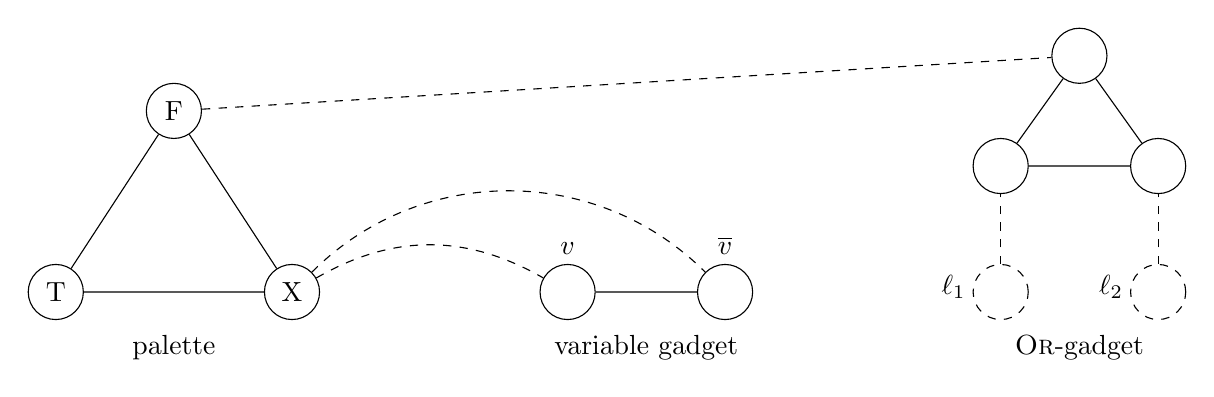
\begin{tikzpicture}[-]
\node[draw, circle, minimum size=.7cm] at (0,0) (p1) {T};
\node[draw, circle, minimum size=.7cm]  at (3,0) (p2) {X};
\node[draw, circle, minimum size=.7cm]  at (1.5,2.3) (p3) {F};
\node [draw=none] at (1.5,-0.7) {palette};
\node[draw, circle, minimum size=.7cm,label=$v$] at (6.5,0) (v1) {};
\node[draw, circle, minimum size=.7cm,label=$\overline{v}$]  at (8.5,0) (v2) {};
\node [draw=none] at (7.5,-0.7) {variable gadget};
\node[draw, circle, dashed, minimum size=.7cm,label={[xshift=-1.7em, yshift=-1.6em] $\ell_1$}] at (12,0) (o1) {};
\node[draw, circle, dashed, minimum size=.7cm,label={[xshift=-1.7em, yshift=-1.6em] $\ell_2$}]  at (14,0) (o2) {};
\node[draw, circle, minimum size=.7cm] at (12,1.6) (o3) {};
\node[draw, circle, minimum size=.7cm]  at (14,1.6) (o4) {};
\node[draw, circle, minimum size=.7cm] at (13,3) (o5) {};
\node [draw=none] at (13,-0.7) {\textsc{Or}-gadget};
\draw 
(p1) -- (p2) -- (p3) -- (p1)
(v1) -- (v2)
(o3) -- (o5) -- (o4) -- (o3)
(o1) edge[below, dashed] node{} (o3)
(o2) edge[below, dashed] node{} (o4)
(p2) edge[bend left, below, dashed] node{} (v1)
(p2) edge[bend left=45, below, dashed] node{} (v2)
(p3) edge[below, dashed] node{} (o5)
;
\end{tikzpicture}

\solution{
\if\isanswerkey1\solThreeColor\fi
To prove that $3COLOR$ is NP-Complete, we first show that $3COLOR \in \NP$. We can build a decider $D_\textnormal{3COLOR}$ that decides $3COLOR$ nondeterministically in polynomial time. The decider $D_\textnormal{3COLOR}$ is defined as following:\\
$D_\textnormal{3COLOR}=$ ``On input $\langle G\rangle$,
\begin{enumerate}
    \item Nondeterministically assign the three color \texttt{F}, \texttt{T}, \texttt{X} to all nodes $V_i$ in graph $G$
    \item Do the following for all assignments
    \item For all node $V_i$ check if all nodes reachable from $V_i$ has different color than $V_i$
    \begin{itemize}
        \item If all nodes' a adjacent nodes have a different color \tmAcc
    \end{itemize}
    \item If no assignments will make all nodes having adjacent node with different color \tmRej''
\end{enumerate}
It is clear that the decider $D_\textnormal{3COLOR}$ runs nondeterministically in polynomial time so that language $3COLOR \in \NP$\\
To show that $\forall A \in \NP \mid A \lep 3COLOR$, we can build a function $f: 3SAT \to 3COLOR$ that runs in polynomial time, which makes $3SAT \lep 3COLOR$. The function $f$ is defined as follow:\\
\begin{enumerate}
    \item On input $\langle\phi(x_1, ..., x_i, ..., x_n)\rangle$, where $\phi$ is a 3CNF formula
    \item Construct graph $G_\phi$ as follow
    \item Make a triangle palette with the node \texttt{T}, \texttt{F} and \texttt{X} that represents \textsc{True}, \textsc{False} and \textsc{Root} as shown below:\\
    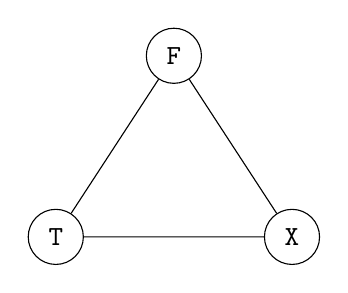
\begin{tikzpicture}[-]
        \node[draw, circle, minimum size=.7cm] at (0,0) (p1) {\texttt{T}};
        \node[draw, circle, minimum size=.7cm]  at (3,0) (p2) {\texttt{X}};
        \node[draw, circle, minimum size=.7cm]  at (1.5,2.3) (p3) {\texttt{F}};
        \draw 
        (p1) -- (p2) -- (p3) -- (p1)
        ;
    \end{tikzpicture}
    \item For each variable $x_i$, create a variables gadget as follow, that connect both node of $x_i$ and $\overline{x_i}$ with the root node in palette, if the value of the variable is \textsc{True} assign it as color \texttt{T}, otherwise assign it as color \texttt{F}\\
    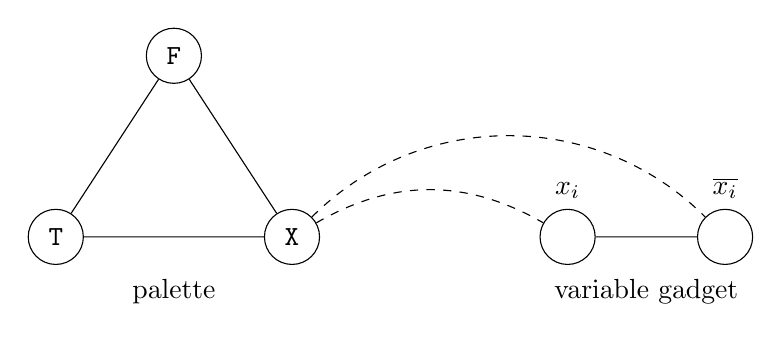
\begin{tikzpicture}[-]
        \node[draw, circle, minimum size=.7cm] at (0,0) (p1) {\texttt{T}};
        \node[draw, circle, minimum size=.7cm]  at (3,0) (p2) {\texttt{X}};
        \node[draw, circle, minimum size=.7cm]  at (1.5,2.3) (p3) {\texttt{F}};
        \node [draw=none] at (1.5,-0.7) {palette};
        \node[draw, circle, minimum size=.7cm,label=$x_i$] at (6.5,0) (v1) {};
        \node[draw, circle, minimum size=.7cm,label=$\overline{x_i}$]  at (8.5,0) (v2) {};
        \node [draw=none] at (7.5,-0.7) {variable gadget};
        \draw 
        (p1) -- (p2) -- (p3) -- (p1)
        (v1) -- (v2)
        (p2) edge[bend left, below, dashed] node{} (v1)
        (p2) edge[bend left=45, below, dashed] node{} (v2)
        ;
    \end{tikzpicture}
    \item For each clause $C_m=(a \vee b \vee c)$, create two Or-gadget as follow:\\
    \begin{tikzpicture}[-]
        \node[draw, circle, minimum size=.7cm] at (0,0) (p1) {\texttt{T}};
        \node[draw, circle, minimum size=.7cm]  at (3,0) (p2) {\texttt{X}};
        \node[draw, circle, minimum size=.7cm]  at (1.5,2.3) (p3) {\texttt{F}};
        \node [draw=none] at (1.5,-0.7) {palette};
        \node[draw, circle, minimum size=.7cm] at (6.5,0) (v1) {$\overline{a}$};
        \node[draw, circle, minimum size=.7cm]  at (8.5,0) (v2) {$a$};
        \node[draw, circle, minimum size=.7cm] at (6.5,-1.5) (v3) {$\overline{b}$};
        \node[draw, circle, minimum size=.7cm]  at (8.5,-1.5) (v4) {$b$};
        \node[draw, circle, minimum size=.7cm] at (6.5,-3) (v5) {$\overline{c}$};
        \node[draw, circle, minimum size=.7cm]  at (8.5,-3) (v6) {$c$};
        \node [draw=none] at (7.5,-5) {variable gadget};
        % \node[draw, circle, dashed, minimum size=.7cm,label={[xshift=-1.7em, yshift=-1.6em] $\ell_1$}] at (12,0) (o1) {};
        % \node[draw, circle, dashed, minimum size=.7cm,label={[xshift=-1.7em, yshift=-1.6em] $\ell_2$}]  at (14,0) (o2) {};
        \node[draw, circle, minimum size=.7cm] at (12,1.6) (o3) {$n_2$};
        \node[draw, circle, minimum size=.7cm]  at (14,1.6) (o4) {$n_3$};
        \node[draw, circle, minimum size=.7cm] at (13,3) (o5) {$n_1$};
        \node[draw, circle, minimum size=.7cm] at (13,-1.4) (o6) {$n_6$};
        \node[draw, circle, minimum size=.7cm]  at (15,-1.4) (o7) {$n_4$};
        \node[draw, circle, minimum size=.7cm] at (14,0) (o8) {$n_5$};
        \node [draw=none] at (14,-3) {\textsc{Or}-gadget};
        \draw 
        (p1) -- (p2) -- (p3) -- (p1)
        (v1) -- (v2)
        (v3) -- (v4)
        (v5) -- (v6)
        (o3) -- (o5) -- (o4) -- (o3)
        (o6) -- (o8) -- (o7) -- (o6)
        (o4) edge[below, dashed] node{} (o8)
        % (o2) edge[below, dashed] node{} (o4)
        (p2) edge[bend left, below, dashed] node{} (v1)
        (p2) edge[bend left=45, below, dashed] node{} (v2)
        (p2) edge[bend right, below, dashed] node{} (v3)
        (p2) edge[bend right=45, below, dashed] node{} (v4)
        (p2) edge[bend right, below, dashed] node{} (v5)
        (p2) edge[bend right=90, below, dashed] node{} (v6)
        (p3) edge[bend left=40, dashed] node{} (o5)
        (p2) edge[bend left=45, dashed] node{} (o5)
        (v2) edge[below, dashed] node{} (o3)
        (v4) edge[below, dashed] node{} (o6)
        (v6) edge[below, dashed] node{} (o7)
        ;
    \end{tikzpicture}
    \item Output $\langle G_\phi\rangle$
\end{enumerate}
For the function $f$, its steps $d, e$ all runs in polynomial time, and other steps are constant time, so that, overall the function $f$ runs in polynomial time. \\
If the $\langle\phi\rangle \in 3SAT$, so that we can fill up the two \textsc{Or}-gadgets having node $n_1$ colored as \texttt{T}, since the node $n_1$ is connected reachable from node \texttt{F} and node \texttt{X}. Consider Boolean variables $a=\textsc{True}$, $b=\textsc{False}$ and $c=\textsc{False}$, the nodes can be colors as shown below such that the node $n_1$ will be colored as \texttt{T}, in this graph $G_\phi$, all adjacent node has a different color, which makes $\langle G_\phi\rangle \in 3COLOR$\\
\begin{tikzpicture}[-]
    \node[draw, circle, minimum size=.7cm] at (0,0) (p1) {\texttt{T}};
    \node[draw, circle, minimum size=.7cm]  at (3,0) (p2) {\texttt{X}};
    \node[draw, circle, minimum size=.7cm]  at (1.5,2.3) (p3) {\texttt{F}};
    \node [draw=none] at (1.5,-0.7) {palette};
    \node[draw, circle, minimum size=.7cm] at (6.5,0) (v1) {\texttt{F}};
    \node[draw, circle, minimum size=.7cm]  at (8.5,0) (v2) {\texttt{T}};
    \node[draw, circle, minimum size=.7cm] at (6.5,-1.5) (v3) {\texttt{T}};
    \node[draw, circle, minimum size=.7cm]  at (8.5,-1.5) (v4) {\texttt{F}};
    \node[draw, circle, minimum size=.7cm] at (6.5,-3) (v5) {\texttt{T}};
    \node[draw, circle, minimum size=.7cm]  at (8.5,-3) (v6) {\texttt{F}};
    \node [draw=none] at (7.5,-5) {variable gadget};
    % \node[draw, circle, dashed, minimum size=.7cm,label={[xshift=-1.7em, yshift=-1.6em] $\ell_1$}] at (12,0) (o1) {};
    % \node[draw, circle, dashed, minimum size=.7cm,label={[xshift=-1.7em, yshift=-1.6em] $\ell_2$}]  at (14,0) (o2) {};
    \node[draw, circle, minimum size=.7cm] at (12,1.6) (o3) {\texttt{F}};
    \node[draw, circle, minimum size=.7cm]  at (14,1.6) (o4) {\texttt{X}};
    \node[draw, circle, minimum size=.7cm] at (13,3) (o5) {\texttt{T}};
    \node[draw, circle, minimum size=.7cm] at (13,-1.4) (o6) {\texttt{T}};
    \node[draw, circle, minimum size=.7cm]  at (15,-1.4) (o7) {\texttt{X}};
    \node[draw, circle, minimum size=.7cm] at (14,0) (o8) {\texttt{F}};
    \node [draw=none] at (14,-3) {\textsc{Or}-gadget};
    \draw 
    (p1) -- (p2) -- (p3) -- (p1)
    (v1) -- (v2)
    (v3) -- (v4)
    (v5) -- (v6)
    (o3) -- (o5) -- (o4) -- (o3)
    (o6) -- (o8) -- (o7) -- (o6)
    (o4) edge[below, dashed] node{} (o8)
    % (o2) edge[below, dashed] node{} (o4)
    (p2) edge[bend left, below, dashed] node{} (v1)
    (p2) edge[bend left=45, below, dashed] node{} (v2)
    (p2) edge[bend right, below, dashed] node{} (v3)
    (p2) edge[bend right=45, below, dashed] node{} (v4)
    (p2) edge[bend right, below, dashed] node{} (v5)
    (p2) edge[bend right=90, below, dashed] node{} (v6)
    (p3) edge[bend left=40, dashed] node{} (o5)
    (p2) edge[bend left=45, dashed] node{} (o5)
    (v2) edge[below, dashed] node{} (o3)
    (v4) edge[below, dashed] node{} (o6)
    (v6) edge[below, dashed] node{} (o7)
    ;
\end{tikzpicture}\\
And if the $\langle\phi\rangle \notin 3SAT$, there is a clause $c_j=(\hat{a}\vee\hat{b}\vee\hat{c})$ that is \textsc{False}. So that $\hat{a}=\hat{b}=\hat{c}=\textsc{False}$. The node will be colored as following\\
\begin{tikzpicture}[-]
    \node[draw, circle, minimum size=.7cm] at (0,0) (p1) {\texttt{T}};
    \node[draw, circle, minimum size=.7cm]  at (3,0) (p2) {\texttt{X}};
    \node[draw, circle, minimum size=.7cm]  at (1.5,2.3) (p3) {\texttt{F}};
    \node [draw=none] at (1.5,-0.7) {palette};
    \node[draw, circle, minimum size=.7cm] at (6.5,0) (v1) {\texttt{T}};
    \node[draw, circle, minimum size=.7cm]  at (8.5,0) (v2) {\texttt{F}};
    \node[draw, circle, minimum size=.7cm] at (6.5,-1.5) (v3) {\texttt{T}};
    \node[draw, circle, minimum size=.7cm]  at (8.5,-1.5) (v4) {\texttt{F}};
    \node[draw, circle, minimum size=.7cm] at (6.5,-3) (v5) {\texttt{T}};
    \node[draw, circle, minimum size=.7cm]  at (8.5,-3) (v6) {\texttt{F}};
    \node [draw=none] at (7.5,-5) {variable gadget};
    % \node[draw, circle, dashed, minimum size=.7cm,label={[xshift=-1.7em, yshift=-1.6em] $\ell_1$}] at (12,0) (o1) {};
    % \node[draw, circle, dashed, minimum size=.7cm,label={[xshift=-1.7em, yshift=-1.6em] $\ell_2$}]  at (14,0) (o2) {};
    \node[draw, circle, minimum size=.7cm] at (12,1.6) (o3) {\texttt{T}};
    \node[draw, circle, minimum size=.7cm]  at (14,1.6) (o4) {\texttt{X}};
    \node[draw, circle, minimum size=.7cm] at (13,3) (o5) {\texttt{F}};
    \node[draw, circle, minimum size=.7cm] at (13,-1.4) (o6) {\texttt{T}};
    \node[draw, circle, minimum size=.7cm]  at (15,-1.4) (o7) {\texttt{X}};
    \node[draw, circle, minimum size=.7cm] at (14,0) (o8) {\texttt{F}};
    \node [draw=none] at (14,-3) {\textsc{Or}-gadget};
    \draw 
    (p1) -- (p2) -- (p3) -- (p1)
    (v1) -- (v2)
    (v3) -- (v4)
    (v5) -- (v6)
    (o3) -- (o5) -- (o4) -- (o3)
    (o6) -- (o8) -- (o7) -- (o6)
    (o4) edge[below, dashed] node{} (o8)
    % (o2) edge[below, dashed] node{} (o4)
    (p2) edge[bend left, below, dashed] node{} (v1)
    (p2) edge[bend left=45, below, dashed] node{} (v2)
    (p2) edge[bend right, below, dashed] node{} (v3)
    (p2) edge[bend right=45, below, dashed] node{} (v4)
    (p2) edge[bend right, below, dashed] node{} (v5)
    (p2) edge[bend right=90, below, dashed] node{} (v6)
    (p3) edge[bend left=40, dashed] node{} (o5)
    (p2) edge[bend left=45, dashed] node{} (o5)
    (v2) edge[below, dashed] node{} (o3)
    (v4) edge[below, dashed] node{} (o6)
    (v6) edge[below, dashed] node{} (o7)
    ;
\end{tikzpicture}\\
In this graph, the two top connected nodes are all colored as \texttt{F}, which violated the rule of language $3COLOR$, so that $\langle G_\phi\rangle \notin 3COLOR$. And then, we have shown that $\langle\phi\rangle \in 3SAT \Longleftrightarrow f(\langle\phi\rangle) \in 3COLOR$. And we also know that function $f$ runs in polynomial time, which makes language $3SAT \lep 3COLOR$. And since we know that $3COLOR \in \NP$. Hence we can conclude that $3COLOR$ is \textsc{NP-Complete}
}



\end{enumerate}




\end{document}
